\section{Syntax}

\subsection{Why Syntax?}

We want to be able to express text or characters in general as 0s and 1s. There are several ways for doing this. These include ASCII, ISO Latin 1, UTF-8 and UTF-16.

\subsubsection{CSV}
CSV stands for comma separated values and is a text representation of tables. On the first line you typically have the headers and on every row you have one record. The problem with CSV is that there are different conventions. Some people use another character than a comma to separate the columns, which limits interoperability. Furthermore, you might need to use certain characters in your table, such as commas, thus you need to find another symbol to use as a separator between columns. If you need a comma in one cell of your tabel, make "quotation marks" around that cell entry. If you need "quotation marks" in your cell, use """tripple quotation"" marks" in your cell.

\subsubsection{Data Denormalization}
As a rule of thumb, normalizing data means joining it back at query time. For data lakes and large-scale data processing, it is often desirable to go exactly the opposite way, called data denormalization. In this case, we can nest data. Data denormalization makes a lot of sense in read-intensive scenarios in which not having to join brings a significant performance improvement. In write-intensive cases, high normal forms make more sense because we want to avoid update anomalies.

A new tool we use for tables that are not in normal form is JSON. A tuple, mathematically a partial mapping function, can be expressed as follows (\cref{lst:json1}). Furthermore, one is also allowed to break relational integrity.

\begin{lstlisting}[style=json, caption={Example JSON code}, label={lst:json1}]
{
    "key": "value",
    "array": [1, 2, 3],
    "nested": {
        "nested_key": "nested_value",
        "nested_table": [
            {"Customer": "John", "quantity": "one"},
            {"Customer": "Peter", "quantity": 2},
            {"Customer": "John"}
        ]
    }
}
\end{lstlisting}

\subsection{Semi-Structured Data and Well-Formedness}
The generic name for denormalized data (in the same of heterogeneous and nested) is “semi-structured data”. Textual formats such as XML and JSON have the advantage that they can both be processed by computers, and can also be read, written and edited by humans. Another very important and characterizing aspect of XML and JSON is that they are standards: XML is a W3C standard. W3C, also known as the World Wide Web consortium, is the same body that also standardizes HTML, HTTP, etc. JSON is now an ECMA stan- dard, which is the same body that also standardizes JavaScript.

When a document is well-formed XML(/JSON), it means that it can be successfully opened by an editor as XML(/JSON) with no errors. On the other hand, a non-well-formed document cannot be used and cannot benefit from all the XML and JSON tools until it is fixed and edited into a well-formed document.

\subsection{JSON}
JSON is made of exactly six building blocks: strings, numbers, Booleans, null, objects, and arrays. Let us go through them.

\subsubsection{Strings}
Strings are simply text. In JSON, strings always appear in double quotes. Obviously, strings could contain quotes and in order not to con- fuse them with the surrounding quotes, they need to be differentiated. This is called escaping and, in JSON, escaping is done with backslash characters ($\backslash$). Other escape sequences include:
\begin{itemize}
    \item $\backslash \backslash$ : $\backslash$
    \item $\backslash$n : new line
    \item $\backslash$r : carriage return
    \item $\backslash$t : tabulation
    \item $\backslash$u followed by four hexadecimal digits : any character (via its Unicode code point)
\end{itemize}

\subsubsection{Numbers}
The way a number appears in syntax is called a lexical representation, or a literal. There are only a few restriction: a leading + is not allowed, a leading 0 is not allowed (with the exception of decimals). In JSON, numbers are unquoted.

\subsubsection{Booleans}
There are two Booleans, true and false, and each one is associated with exactly one possible literal, which are, well, true and false. Booleans are also unquoted.

\subsubsection{Null}
There is a special value, null, which corresponds to the (unique) literal. Some like to see this as an unknown or hidden value, others as equivalent to an absent value, etc. In this course, on the logical level, we will consider that an absent value is not the same thing as a null value.
Null literals are unquoted. Otherwise, they would be recognized as strings by the parser and not as nulls.

\subsubsection{Arrays}
Arrays are simply lists of values. The members of an array can be any JSON value: string, number, Boolean, null, array, or object. They are listed within square brackets, and are separated by commas.
\begin{lstlisting}[style=json, caption={Examples of Arrays}, label={lst:json2}]
[1,2,3]
[ ]
[null,"foo",12.3,false,[1,3]]
\end{lstlisting}

\subsubsection{Objects}
Objects are simply maps from strings to values. The keys of an object must be strings and thus must be quoted. The values associated with them can be any JSON value: string, number, Boolean, null, array, or object. The pairs are listed within curly brackets, and are separated by commas. Within a pair, the value is separated from the key with a colon character. The JSON standard recommends for keys to be unique within an object.
\begin{lstlisting}[style=json, caption={Examples of Objects}, label={lst:json2}]
{ "foo" : 1 }
{}
{ "foo" : "foo", "bar" : [ 1, 2 ],
  "foobar":[{"foo":null}, {"foo":true}]
}   
\end{lstlisting}


\subsection{XML}
XML stands for eXtensible Markup Language. It resembles HTML, except that it allows for any tags and that it is stricter in what it allows. XML is considerably more complex than JSON but, fortunately, most datasets only use a subset of what XML can do. In our course, we will stick to the most common features of XML. XML’s most important building blocks are elements, attributes, text and comments.

\subsubsection{Elements}
XML is a markup language, which means that content is “tagged”. Tagging is done with XML elements. An XML element consists of an opening tag, and a closing tag. What is “tagged” is everything inbetween the opening tag and the closing tag.

\begin{lstlisting}[style=xml, caption={Example XML code}, label={lst:xml1}]
<person>(any content here)</person>
<!-- If there is no content at all, we can write empty elements with a simple tag -->
<person/>
<!-- which is equivalent to -->
<person></person>
<!-- Elements nest arbitrarily -->
<person><first>(some content)</first><student/>
<last>(some other content)</last></person>
<!-- It is possible to use indentation and new lines to pretty- print the document for ease of read by a human: -->
<person>
  <first>(some content)</first>
  <student/>
  <last>(some other content)</last>
</person>
c
<persons>
  <person>
    <first>(some content)</first>
    <last>(some other content)</last>
  </person>
  <person>
    <first>(some content)</first>
    <last>(some other content)</last>
  </person>
  <person>
    <first>(some content)</first>
    <last>(some other content)</last>
  </person>
</persons>
\end{lstlisting}
Inner elements must be closed before the outer elements. A well-formed XML document must have exactly one element.

\subsubsection{Attributes}
Attributes are key-value pairs. Attributes can be double quoted or single quoted. The key is never quoted and there cannot be duplicate keys. Attributes can also appear in empty element tags, but cannot appear in a closing tag. Furthermore, elements canno tnest within attribute values. And lastly, attributes are not allowed to start with XML or xml or any combinatino.

\begin{lstlisting}[style=xml, caption={Example XML code}, label={lst:xml2}]
<person birth="1879" death='1955'>
    <first>(some content)</first>
    <last>(some other content)</last>
</person>
\end{lstlisting}

\subsubsection{Text}
Text is freely appearing in elements and without any quotes (attribute values are not text!). E.g.
\begin{lstlisting}[style=xml, caption={Example XML code}, label={lst:xml3}]
<person birth="1879" death="1955">
    <first>Albert</first>
    <last>Einstein</last>
</person>
<!-- Text cannot appear on its own at the top level. This is wrong: -->
Albert <person/> Einstein
<!-- Within an element, text can freely alternate with other elements, called mixed content. This is unique to XML -->
<person>
    <style>His Royal Highness</style>
    The <title>Duke of <location>Cambridge</location></title>
</person>
\end{lstlisting}

\subsubsection{Comments}
Examples of comments have been seen in the previous example blocks. However, a single comment is not well-formed XML (remember: we need exactly one top-level element). Comments can also appear at the top-level though, but under the condition that there is exactly one top-level element.
\begin{lstlisting}[style=xml, caption={Example XML code}, label={lst:xml4}]
<person birth="1879" death="1955">
    <first>Albert</first>
    <last>Einstein</last>
    <!-- He is still famous today -->
</person>
\end{lstlisting}

\subsubsection{Text declaration}
XML documents can be identified as such with an optional text decla- ration containing a version number and an encoding.
\begin{lstlisting}[style=xml, caption={Example XML code}, label={lst:xml5}]
<?xml version="1.0" encoding="UTF-8"?>
<person birth="1879" death="1955">
    <first>Albert</first>
    <last>Einstein</last>
</person>
\end{lstlisting}
Another tag that might appear right below, or instead of, the text declaration is the doctype declaration. It must then repeat the name of the top-level element, like so:
\begin{lstlisting}[style=xml, caption={Example XML code}, label={lst:xml6}]
<?xml version="1.0" encoding="UTF-8"?>
<!DOCTYPE person>
<person birth="1879" death="1955">
    <first>Albert</first>
    <last>Einstein</last>
</person>
\end{lstlisting}

\subsubsection{Summary}

\begin{table}[H]
    \centering
    \begin{tabular}{|c|c|c|c|}
        \hline
         & Top-Level & Between Element Tags & Inside Opening Element Tag \\ \hline
        Elements & once & yes & no \\ \hline
        Attributes & no & no & yes \\ \hline
        Text & no & yes & no \\ \hline
    \end{tabular}
    \caption{What appears where?}\label{tab:Waw}
\end{table}

\subsubsection{Escaping special characters}
In XML escaping is done with an ampersand (\&) character. There are exactly five possible escape sequences pre-defined in XML:
\begin{table}[H]
    \centering
    \begin{tabular}{cc}
        \hline
        Escape sequence & Corresponding character \\ \hline
        \&lt; & $<$ \\
        \&gt; & $>$ \\
        \&quot; & " \\
        \&apos; & ' \\
        \&amp; & \& \\ \hline
    \end{tabular}
    \caption{Escape characters}\label{tab:escchar}
\end{table}
Escape sequences can be used anywhere in text, and in attribute values. At other places (element names, attribute names, inside comments), they will not be recognized or will lead to well-formedness errors.
In text, \& and $<$ must(!) be escaped. The other characters may, but need not to, be escaped. In double-quoted attribute values ",\& and $<$ must(!) be escaped. The other characters may, but need not to, be escaped. In single-quoted attribute values ',\& and $<$ must(!) be escaped. The other characters may, but need not to, be escaped.

\subsubsection{XML Names}
There are a few rules how one can name an element.
\begin{itemize}
    \item An element name may not start with a digit. (wrong: $<$1234/$>$)
    \item An element name may not contain the $<$ sign and one cannot escape it. (wrong: $<$a$<$b/$>$)
    \item An element may not be named xml (by the user, developers of the service may use it, no matter the spelling (capitalized, not capitalized, mixed capitalization)). (wrong: $<$xml/$>$)
\end{itemize}

\begin{figure}[h]
    \centering
    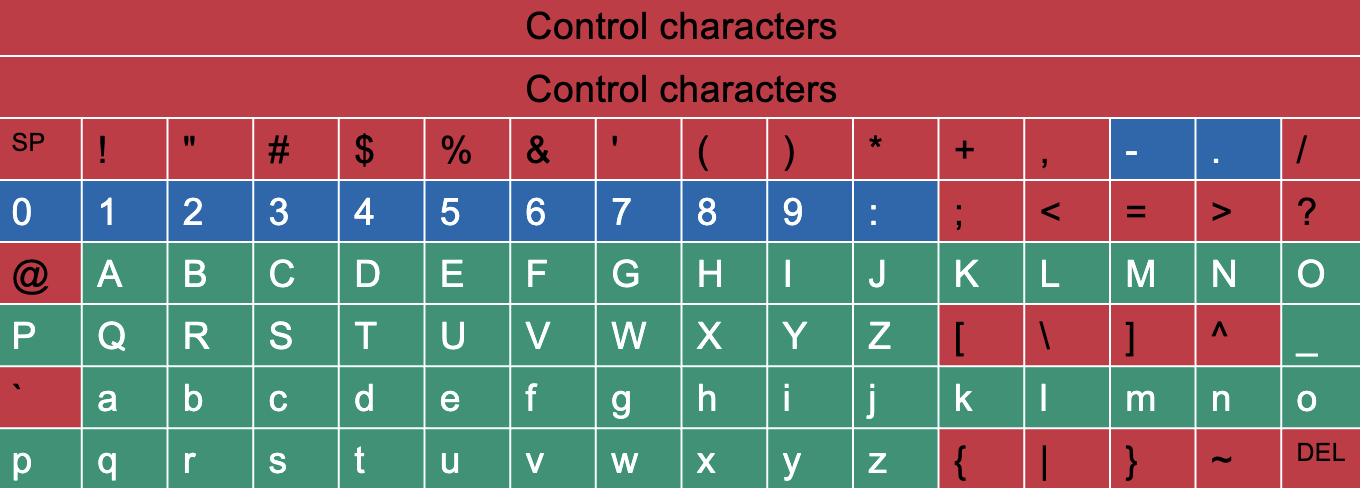
\includegraphics[width=0.7\textwidth]{Figures/CharactersAllowed.png}
    \caption{ASCII characters allowed in XML names. \textcolor{darkgreen}{Green: Allowed anywhere in name}, \textcolor{darkblue}{Blue: allowed but not at the start}, \textcolor{darkred}{Red: not allowed}.}\label{fig:charallow}
\end{figure}

\subsubsection{Namespaces in XML}

\textcolor{grey}{(Not so relevant for the exam. Only important to know that they exist.)}

When a lot of data is created in the XML format, scaling issues start appearing because people use the same element and attribute names for different purposes. For example, an element named "client" can be used in customer relationship datasets, or in computer network datasets.
Namespaces are an extension of XML that allows users to group their elements and attributes in packages, similar to Python modules, Java packages or C++ namespaces. This is a very natural thing to do.

A namespace is identified with a URI. XML namespaces start with \textit{http://} . It is possible to put all elements of an XML document in a namespace. E.g.

\begin{lstlisting}[style=xml, caption={Example XML code}, label={lst:xml7}]
<persons xmlns="http://www.example.com/persons">
  <person>
    <first>(some content)</first>
    <last>(some other content)</last>
  </person>
  <person>
    <first>(some content)</first>
    <last>(some other content)</last>
  </person>
  <person>
    <first>(some content)</first>
    <last>(some other content)</last>
  </person>
</persons>
\end{lstlisting}
In the above document, the elements person, first and last all live in the namespace http://www.example.com/persons. xmlns is not an attribute, it is really a namespace declaration. Remember, we saw that attributes starting with xml are forbidden, and this is because this is reserved for namespace declarations. We say that the namespace is absent for these elements, if there is no declaration of a namespace.

\paragraph{QNames}
What about documents that use multiple namespaces? This is done by associating namespaces with prefixes, which act as shorthands for a namespace. Then, we can use the prefix shorthand in every element that we want to have in this namespace.

\begin{lstlisting}[style=xml, caption={Example XML code}, label={lst:xml8}]
<m:math xmlns:m="http://www.w3.org/1998/Math/MathML">
<m:apply>
    <m:eq/>
    <m:ci>x</m:ci>
    <m:apply>
    <m:root/>
    <m:cn>2</m:cn>
    </m:apply>
</m:apply>
</m:math>
\end{lstlisting}

In the above example, \texttt{m} is called the local name of the element.


\subsubsection{Datasets in XML}
A table can be stored as follows:

\begin{lstlisting}[style=xml, caption={Example XML code}, label={lst:xml9}]
<sales>
  <sale>
    <product>Phone</product>
    <price>800</price>
    <customer>John</customer>
    <quantity>1</quantity>
  </sale>
  <sale>
    <product>Phone</product>
    <price>800</price>
    <customer>Peter</customer>
    <quantity>2</quantity>
  </sale>
  <sale>
    <product>Phone</product>
    <price>800</price>
    <customer>Mary</customer>
    <quantity>1</quantity>
  </sale>
  <sale>
    <product>Laptop</product>
    <price>200</price>
    <customer>John</customer>
    <quantity>3</quantity>
  </sale>
</sales>
\end{lstlisting}

A nested table may look like:

\begin{lstlisting}[style=xml, caption={Example XML code}, label={lst:xml10}]
<?xml version "1.0"?>
<!DOCTYPE sales>
<sales>
  <sale>
    <product>Phone</product>
    <price>800</price>
    <orders>
      <order>
        <customer>John</customer>
        <quantity>1</quantity>
      </order>
      <order>
        <customer>Peter</customer>
        <quantity>2</quantity>
      </order>
      <order>
        <customer>Mary</customer>
        <quantity>1</quantity>
      </order>
    </orders>
  </sale>
</sales>
\end{lstlisting}
